\documentclass[mathserif]{beamer}
\usepackage[utf8]{inputenc}
\usepackage{amsmath}
\usepackage{amsfonts}
\usepackage{amssymb}
\usepackage{arydshln}
\usepackage{graphicx}
\usepackage{float}
\usepackage{picture}
\usepackage{dcolumn}
\usepackage{textpos}
\usepackage{graphicx}

\setbeamercolor{structure}{fg=grey}
\usetheme[sectionpage=progressbar, progressbar=frametitle]{metropolis}

\definecolor{prettyBlue}{HTML}{2196F3}
\setbeamercolor{progress bar}{fg=prettyBlue, bg=gray}

%Information to be included in the title page:
\title{Development of a Pendulum Control System}
\author{Thomas S. Christensen \\ Mikkel S. Jaedicke\\}

\institute{University of Southern Denmark}
\date{Jan, 2018} 

\addtobeamertemplate{frametitle}{}{%
\begin{textblock*}{200mm}(\textwidth-1.5cm,-0.8cm)

\includegraphics[scale=0.15]{graphics/sdu_logo}
\end{textblock*}}

\begin{document}

\begin{frame}[t]\frametitle{~}
\maketitle
\end{frame}

\begin{frame}[t]\frametitle{title}
    
\centering
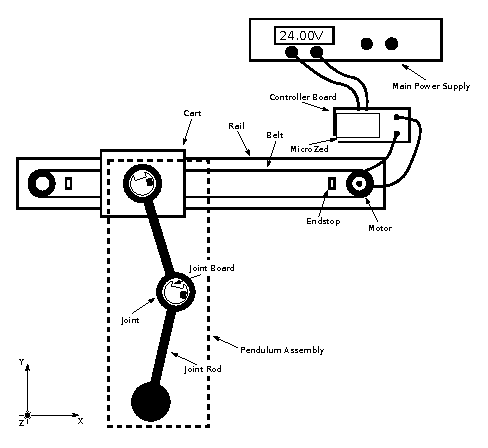
\includegraphics[scale=1]{graphics/system_overview}
\end{frame}

\begin{frame}{First Frame}
Hello, world!
\pause
Hello, world!
\end{frame}

\begin{frame}[c]\frametitle{Workflow}
\centering
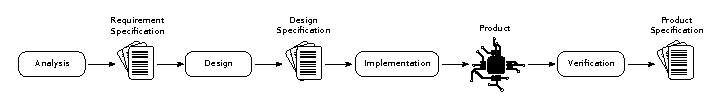
\includegraphics[width=\textwidth]{graphics/workflow}    
\end{frame}

\begin{frame}[standout]
  Questions?
\end{frame}

\end{document}